%\documentclass[fleqn, letterpaper]{amsart}
\documentclass[letterpaper]{tufte-handout}
\usepackage{times}
\usepackage{amsmath}
\usepackage{amssymb}
\usepackage{graphicx}
\usepackage{booktabs}
\usepackage{multirow}
\usepackage{listings}
\usepackage{epstopdf}
\usepackage{bm}
\usepackage{natbib}
%\usepackage[left=1in]{geometry}

\newcommand{\R}{\mathcal{R}}
\newcommand{\E}{\text{E}}
\newcommand{\p}{p_{XY}}
\newcommand{\T}{^\text{T}}
\newcommand{\y}{\mathbf{y}}
\newcommand{\z}{\mathbf{z}}
\newcommand{\I}{\mathbf{I}}
\newcommand{\HH}{\mathbf{H}}
\newcommand{\A}{\mathbf{A}}
\newcommand{\GG}{\mathbf{G}}
\newcommand{\vecv}{\mathbf{v}}
\newcommand{\uu}{\mathbf{u}}
\newcommand{\cyy}{\mathbf{C}_{yy}}
\newcommand{\cyz}{\mathbf{C}_{yz}}
\newcommand{\czz}{\mathbf{C}_{zz}}
\newcommand{\cuu}{\mathbf{C}_{uu}}
\newcommand{\cvv}{\mathbf{C}_{vv}}
\newcommand{\cpp}{\mathbf{C}_{\psi\psi}}
\renewcommand{\arraystretch}{1.5}
\newcommand{\KK}{\left(\begin{array}{c} \frac{{\sigma_{\y_1}}^2}{{\sigma_v}^2 + {\sigma_{\y_1}}^2}\\ \frac{\sigma_{\y_1\y_2}}{{\sigma_v}^2 + {\sigma_{\y_1}}^2} \end{array}\right)}
\newcommand{\cyylong}{\left(\begin{array}{cc} {\sigma_{y_1}}^2 & \sigma_{\y_1\y_2}\\ \sigma_{\y_1\y_2} & {\sigma_{y_2}}^2 \end{array}\right)}
\renewcommand{\vec}[1]{\mathrm{#1}}

\title{Course Project --- ENCE689E Spring 2014}
\author{David Prentiss}

\begin{document}
\maketitle

\section{Herd Dynamics Model}
xra
\section{The Forward Model}
euanoehud aoeuaoeu aeuaoeu aoeuao euao uao eua oe uao uao ua ouao neuhasou aonsuha ehtuas ouhaos uahotneuh 
{\scriptsize
                \lstinputlisting[language=Matlab, caption={Herd ensemble forwar model},
                basicstyle=\ttfamily, label=lst1]{herd.m}
}

See figures \ref{rfe} and \ref{ensemble}.
\begin{figure}
        \includegraphics[width=\textwidth]{rfe}
        \caption{Rainfall realization generated by random walk}
        \label{rfe}
\end{figure}
\begin{figure}
        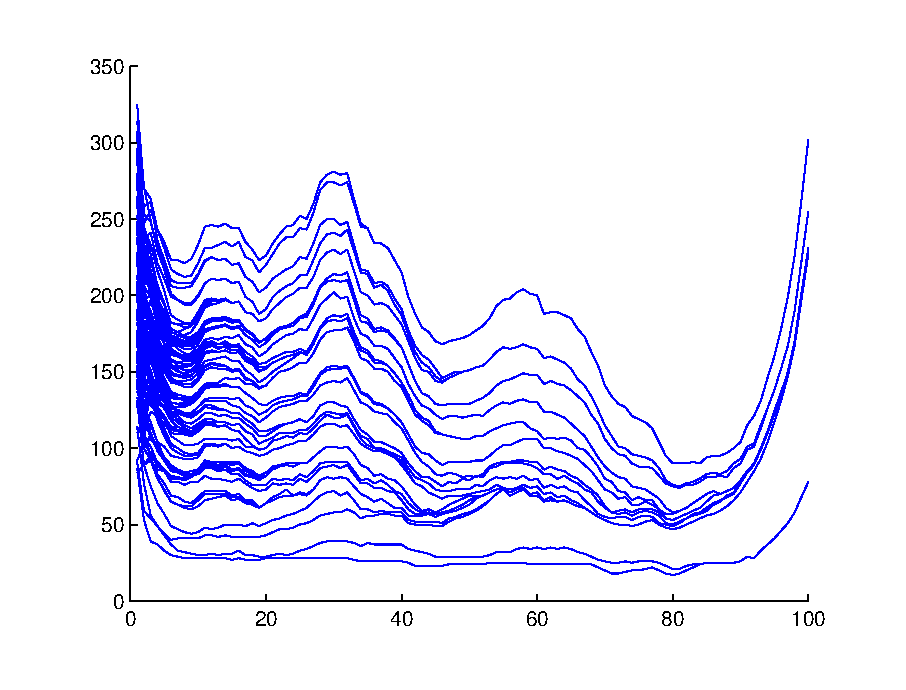
\includegraphics[width=\textwidth]{herdsize}
        \caption{Herd sizes of a 100-member ensemble propogated over 100 seasons.}
        \label{ensemble}
\end{figure}
\end{document}